\section{Architettura}
\subsection{Server di Bootstrap}
Il server di bootstrap deve permettere l'accesso (e l'uscita) dei peer e dei superpeer alla (e dalla) rete P2P, fornendo loro gli indirizzi di alcuni superpeer attivi nella rete (se presenti). Inoltre è suo compito mantenere le informazioni relative ai superpeer attivi attraverso una lista, nella quale memorizza il loro indirizzo IP, e un campo intero ad esso associato (TTL). Tale campo viene utilizzato per verificare la permanenza del superpeer nella rete. \linebreak
Il server svolge il suo lavoro in maniera concorrenziale, tramite l'utilizzo del multiplexing, implementato nel codice con la chiamata di sistema select.\linebreak
I descrittori controllati nella select del server sono illustrati in figura \ref{select_server}:

\begin{figure}[htpb]
\centering
{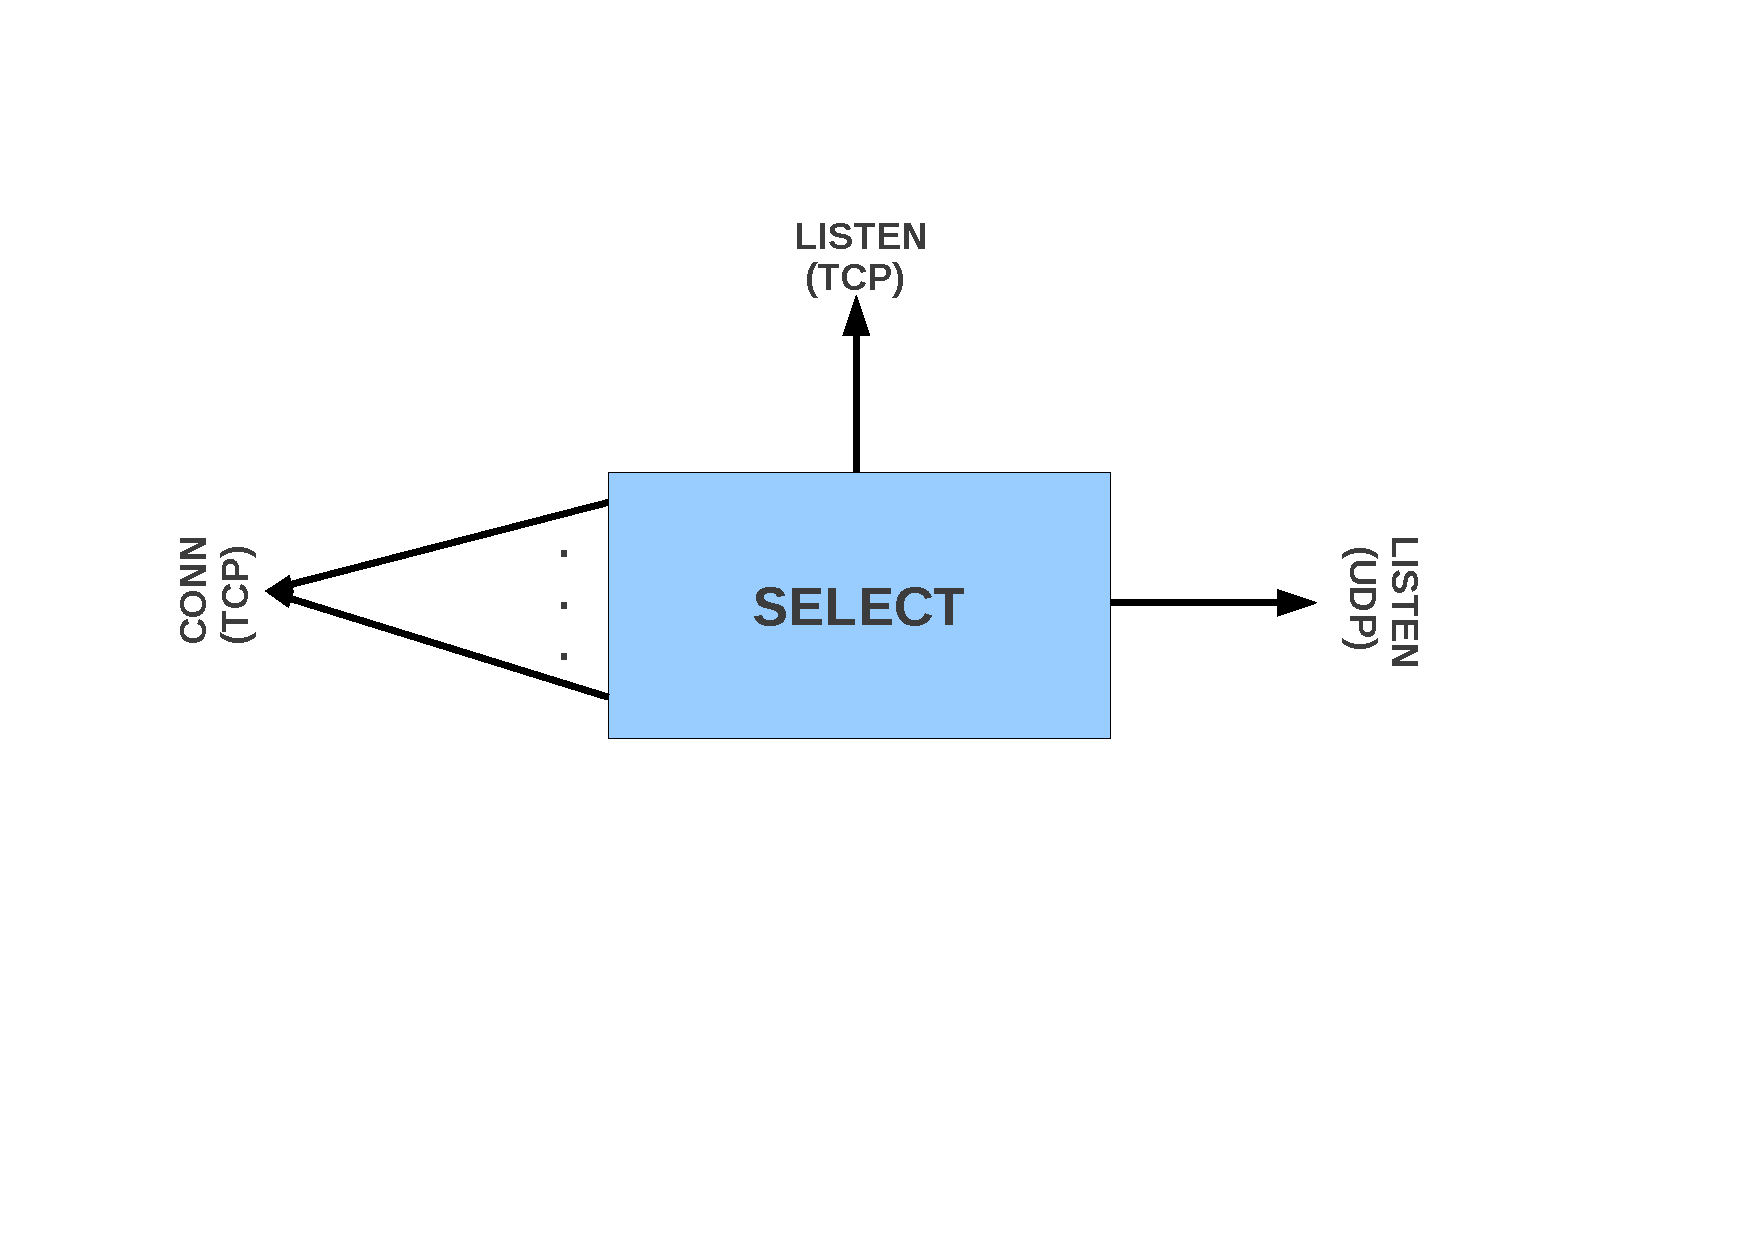
\includegraphics[width=10cm]{img/Select_bootstrap}}
\caption{Struttura select del server\label{select_server}}
\end{figure}

Il listen (TCP) è il descrittore della socket in attesa di connessioni entranti. Quando questo descrittore è pronto in lettura vuol dire che è arrivata una richiesta di connesione, la quale deve essere accettata dal server, instaurando così una connessione TCP. Il descrittore della socket relativo a tale connesione viene inserito sia tra i descrittori da controllare nella select, sia in una lista locale che mantiene tutti i descrittori delle connessioni accettate, in attesa di essere servite.\linebreak
I conn (TCP) sono i descrittori delle connessioni TCP già instaurate e in attesa di servizio.
Quando un descrittore di tipo conn è pronto in lettura significa che è stato ricevuto un messaggio dal server che può essere di 3 tipi:

\begin{itemize}
\item Join;
\item Register;
\item Leave;
\end{itemize}

Una volta letto il messaggio, il server servirà il client e successivamente verrà eliminato dalla select il descrittore della socket relativo alla sua connessione. Se non ci sono altri descrittori pronti in lettura, il server torna in attesa che si sblocchi un qualunque descrittore presente nella select.\linebreak
Il descrittore della socket listen (UDP)  è sempre in attesa di messaggi di tipo "ping" da parte dei superpeer attivi: ogni volta che questo descrittore è pronto in lettura, il server verifica se il messaggio ricevuto è effettivamente un "ping". In caso affermativo, reimposta il TTL del superpeer (al suo valore massimo, ossia 5) dal quale ha ricevuto il messaggio.\linebreak  

\subsection{Superpeer}
Il superpeer ha un' architettura piuttosto complessa in quanto deve gestire sia la comunicazione con altri superpeer che quella con i peer a lui collegati.\linebreak
\subsubsection{Struttura select superpeer}
Per gestire le comunicazioni in modo efficente e simulare la concorrenzialità, il superpeer utilizza il multiplexing, implementato nel codice tramite la select.\linebreak
La select del superpeer deve gestire principalmente 2 socket di ascolto (una per l'UDP e una per il TCP) e un numero variabile (configurabile da file config) di socket di connessione TCP, relative alle connessioni con altri superpeer.\linebreak
Si riporta in figura \ref{select_superpeer} i descrittori controllati nella select.

\begin{figure}[htpb]
\centering
{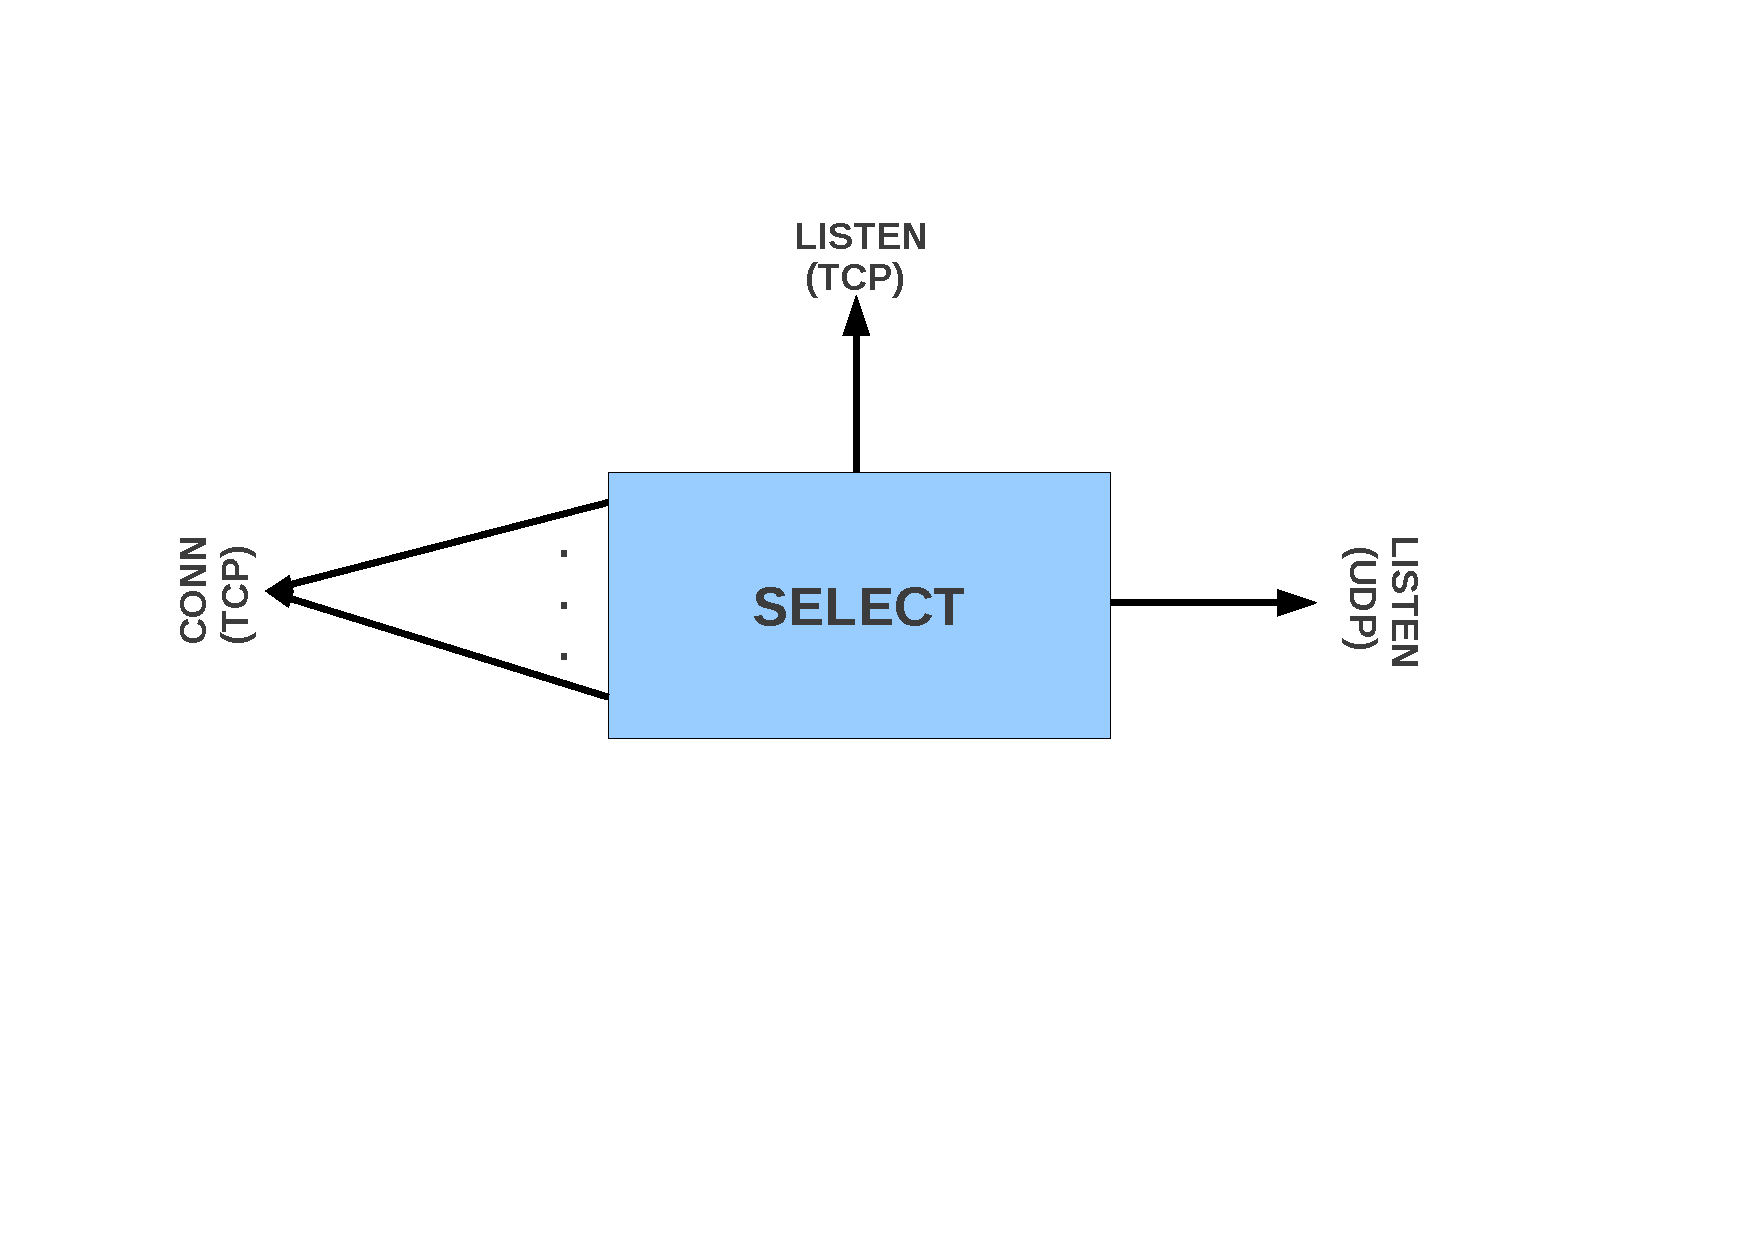
\includegraphics[width=10cm]{img/Select_bootstrap}}
\caption{Select del superpeer\label{select_superpeer}}
\end{figure}
Il descrittore di listen (TCP) è pronto in lettura quando c'è la richiesta di instaurazione di una connessione TCP da parte di un altro superpeer: se il superpeer che riceve la richiesta non ha raggiunto il numero massimo di connessioni disponibili per collegarsi con altri superpeer, accetterà la connessione inviando un pacchetto con comando uguale ad "ack". I due superpeer così connessi si scambieranno informazioni sulle rispettive statistiche di occupazione a livello di rete overlay (numero superpeer connessi) e su quanti peer possiede ciascuno di loro. Quando la listen (TCP) è pronta in lettura, se il superpeer ha esaurito le connessioni disponibili per la rete overlay, accetterà comunque la connessione TCP    e cercherà nella sua lista di superpeer vicini se c'è qualcuno di loro che non sia pieno; se presenti, creerà un pacchetto con comando "full" e campo dati contenente gli indirizzi dei superpeer liberi. A questo punto, viene chiusa la connessione TCP e il superpeer che ha iviato la richiesta di connessione e che riceve un pacchetto con comando "full", dopo aver verificato che la dimensione del campo dati sia diversa da zero, parserà quel campo e contatterà gli indirizzi dei superpeer restituiti, al fine di instaurare una connessione TCP.\linebreak
Il descrittore di listen (UDP) è pronto in lettura quando riceve un messaggio da un peer, oppure quando riceve una risposta/richiesta ad/di una whohas da superpeer che non sono suoi vicini (non direttamente collegati in TCP).I messaggi che si possono essere ricevuti su questa socket sono i seguenti:\linebreak

Dai peer:
\begin{itemize}
\item Join;
\item Whohas;
\item Leave;
\item Elezione;
\item Riscontri relativi all'elezione "ackE", "nakE";
\item Ping;
\item Stop;
\end{itemize}

Dai superpeer:
\begin{itemize}
\item Whohas;
\item Ack;
\end{itemize}

Le azioni che il superpeer intraprende quando riceve uno dei suddetti messaggi verranno spiegate nei capitoli appositi.\linebreak
I descrittori di conn (TCP) sono in attesa di messaggi provenienti dalla rete di overlay, in particolare dai vicini del superpeer.\linebreak
I possibili messaggi che possono rendere pronto in lettura uno di questi descrittori sono i seguenti:\linebreak

\begin{itemize}
\item Whohas;
\item Ack;
\item Merge(fusione);
\item ackM riscontro per il messaggio di fusione;
\item ping;
\item lettura di 0 byte (che equivale a dire che il superpeer corrispondente a questa socket ha interrotto la connessione);
\end{itemize}

Anche in questo caso le azioni intraprese dal superpeer alla ricezione di questi messaggi verranno specificate in seguito.

\subsubsection{Protocolli di comunicazione}
Il superpeer utilizza come protocollo di trasporto sia UDP che TCP. Per la comunicazione con i peer è stato scelto di utilizzare l'UDP in quanto ogni superpeer ha in generale molti peer a lui connessi e di conseguenza si è optato per un protocollo che richiede meno risorse e lo scambio di un numero minore di messaggi per la comunicazione (rispetto al TCP).\linebreak
Per le connessioni nella rete overlay si sono utilizzati entrambi i protocolli TCP e UDP: il TCP è usato per instaurare connessioni permanenti con dei superpeer(che chiameremo vicini), mentre l'UDP è utilizzato durante le whohas per inoltrare le richieste (o risposte) ai superpeer che non sono vicini, i cui indirizzi sono ottenuti nelle risposte alla whohas ricevute dai superpeer vicini (come si spiegherà in dettaglio nel capitolo riguardante la fase di lookup).\linebreak
La scelta dell'utilizzo congiunto di TCP e UDP per la rete di overlay è stata fatta in base alla necessità di avere la trasmissione affidabile propria del TCP almeno con i superpeer vicini, che sono un numero limitato. D'altra parte,l'UDP è stato scelto per la comunicazione tra superpeer che non sono vicini poichè i messaggi che vengono scambiati tra di loro appartengono esclusivamente alla fase di lookup; questa potrebbe richiedere il bisogno di contattare numerosi superpeer e di conseguenza sarebbe eccessivamente pesante per la rete  overlay l'utilizzo del TCP. Inoltre in questa fase si è ritenuto accettabile la perdita di alcuni pacchetti di risposta o di inoltro delle whohas, in quanto in situazione di regime si possono contattare un numero elevato di superpeer.\linebreak


\subsection{Peer}
L'architettura del peer è piuttosto articolata, poichè deve gestire in modo concorrenziale le seguenti attività:
\begin{itemize}
\item Funzionalità principali del peer: menu e gestione dei comandi;
\item Upload;
\item Controllo
\end{itemize}
Ci sono quindi tre processi per gestire in modo separato questi compiti (figure \ref{arc_peer}). 
\begin{figure}[h]
\centering
{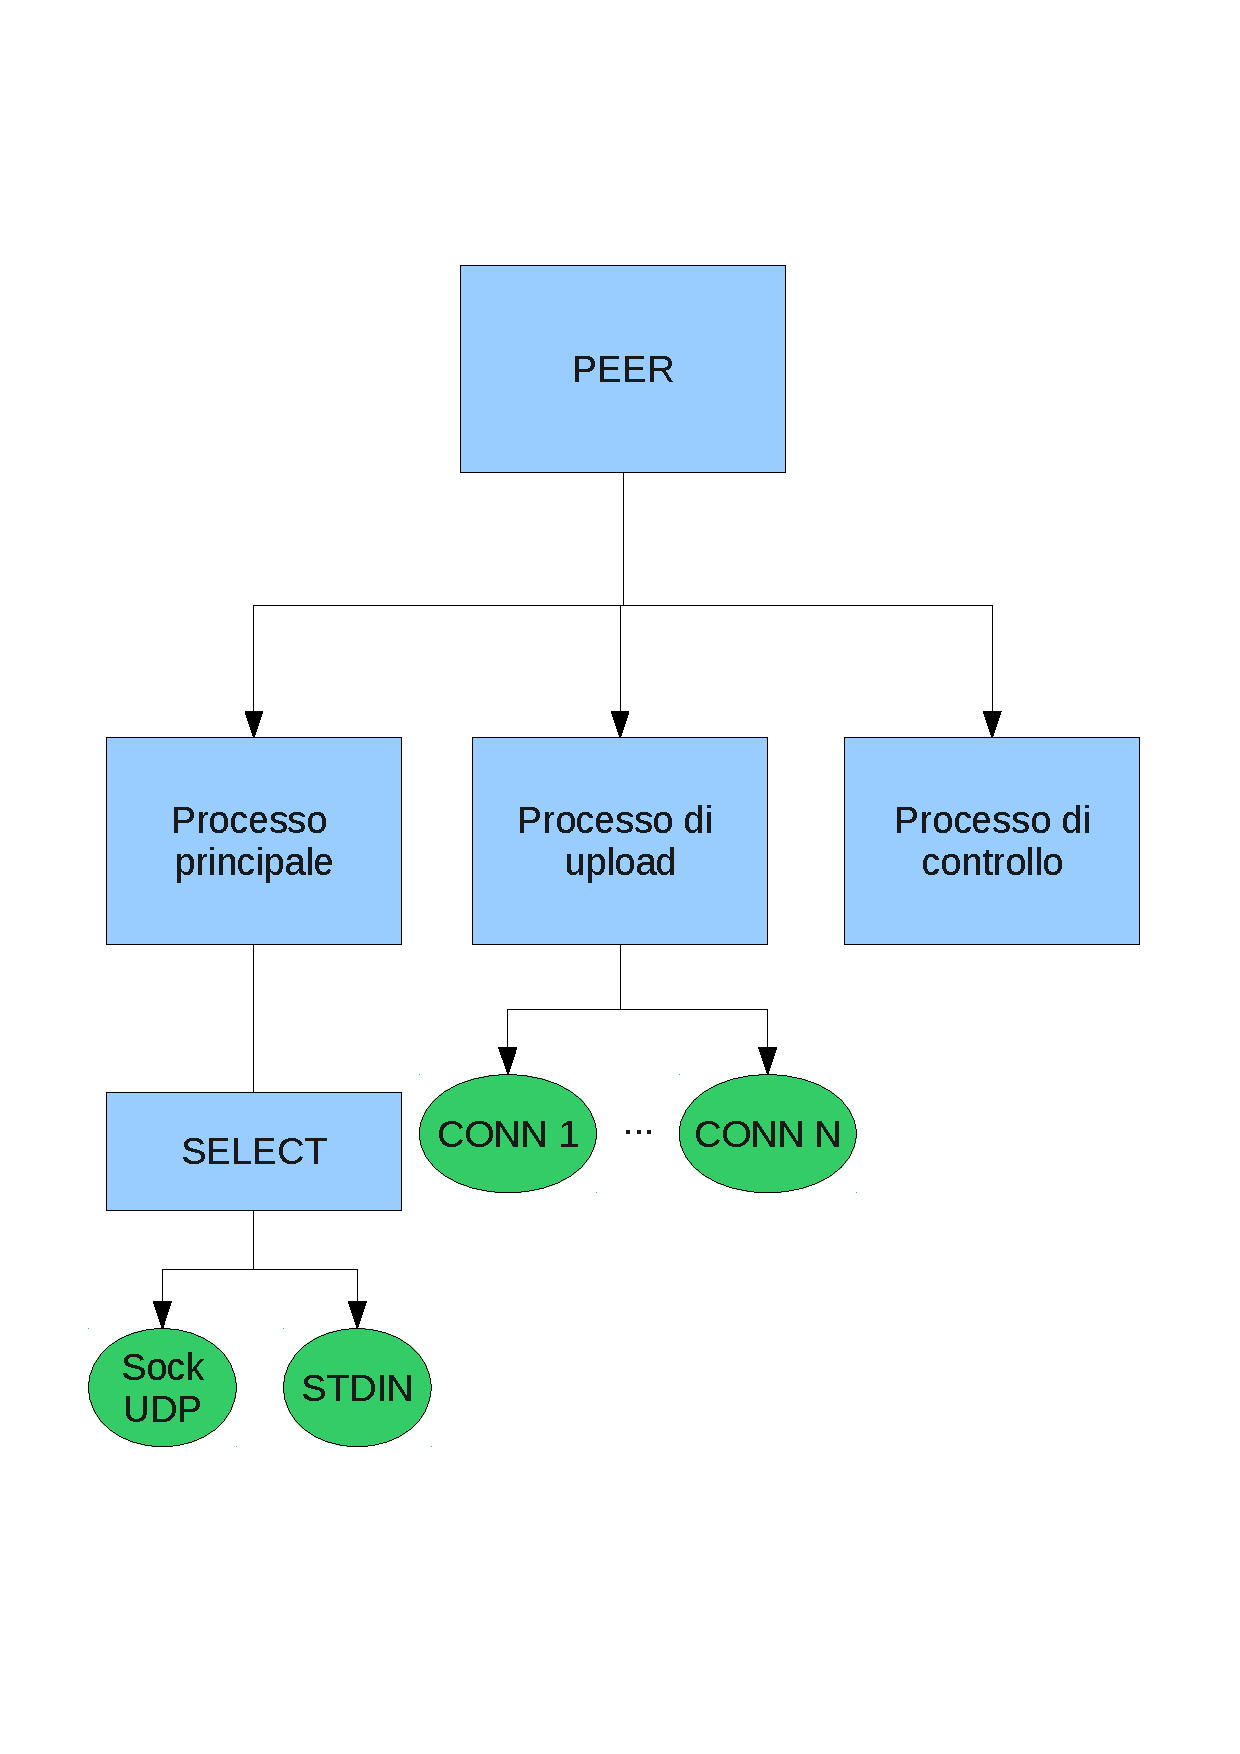
\includegraphics[width=7cm]{img/architettura_peer}}
\caption{Architettura del peer\label{arc_peer}}
\end{figure}
\subsubsection{Processo principale del peer}
È il processo più importante del peer, in quanto permette all'utente di interagire con la rete. \linebreak
A parte i processi di upload e di controllo, il peer svolge il suo lavoro in maniera concorrenziale, utilizzando il multiplexing, implementato nel codice con la chiamata di sistema select.\linebreak
La select gestirà due descrittori:
\begin{itemize}
\item Il descrittore della socket UDP per poter inviare/ricevere messaggi al/dal superpeer
\item Il descrittore dello stdin per poter gestire le richieste immesse dall'utente da tastiera
\end{itemize}
Il descrittore della socket UDP sarà attivato quando verrà ricevuto un messaggio UDP dal superpeer. I messaggi che il peer può ricevere dal superpeer sono:
\begin{itemize}
\item Stop
\item Leave
\item Nwsp
\item Ack
\end{itemize}
Il messaggio di stop e di ack sono messaggi inerenti ai risultati di una ricerca precedentemente fatta dal peer. Il primo identifica il fatto che il superpeer ha bloccato la ricerca e lo comunica al peer. Il messaggio di ack invece identifica una lista di ip, ricevuti in risposta ad una ricerca, dai quali scaricare il file cercato.\linebreak
Il messaggio di nwsp da parte del superpeer implica che il peer che lo riceve è stato eletto superpeer, quindi tale peer avvierà il processo di superpeer e si connetterà ad esso.\linebreak
Se un superpeer invia un messaggio di leave al peer vuol dire che si sta sconnettendo dalla rete; il peer avrà quindi la necessità di connettersi ad un nuovo superpeer e sarà proprio il superpeer che si sconnette a consigliare al peer a chi connettersi.
\linebreak\linebreak
Il descrittore dello stdin sarà attivato quando verrà ricevuto un input da tastiera. Il menu fornisce le seguenti scelte:
\begin{itemize}
\item Leave
\item Update
\item Whohas
\item Stop
\end{itemize}
L'utente può avviare ricerce (whohas) e fermarle (stop) quando ha ricevuto qualche risultato, aggiornare i suoi dati sul superpeer (update), e, quando decide di uscire dalla rete, effettuare il comando apposito (leave)
\subsubsection{Processo di upload}
Questo processo si occupa di servire le richieste di download provenienti da altri peer e di conseguenza c'è una porta TCP perennemente in ascolto. Quando arriva una richiesta di download, il processo sul quale è attiva la socket in ascolto, se non si stanno già servendo il numero massimo di richieste, accetterà la connessione e avvierà un processo specifico per il download del file, il quale, una volta terminato, manderà un segnale al processo padre, così da aggiornare il numero di connessioni attive. \linebreak
I dettagli delle procedure di download e upload verranno illustrati nel capitolo "Fase di download".	\linebreak
\subsubsection{Processo di controllo}
Il processo di controllo effettua periodicamente due operazioni: controlla se il processo main si è chiuso (in caso affermativo chiude tutti i processi del peer che non è più in esecuzione) e si occupa di inviare in modo ciclico un segnale di tipo SIGUSR1 al processo principale, al fine di temporizzare l'operazione di ping. Ogni volta che il processo principale riceverà questo segnale, effettuerà la specifica procedura di ping\_handler.\linebreak
La funzione di ping\_handler è molto importante perchè notifica al superpeer che il peer è ancora attivo e gli permette anche di comunicare il suo rating a quel dato istante. \linebreak
La necessità di comunicare il rating periodicamente al superpeer è dovuta dalla natura dinamica della variabile rating, la quale è molto importante per la gestione dinamica della rete, poichè attraverso di essa si cerca di eleggere sempre superpeer migliori e più stabili.\linebreak
La variabile rating è somma di due fattori: caratteristiche del peer e quantità di tempo trascorsa da quando esso è connesso alla rete.\linebreak
Il rating dato dalle caratteristiche del peer è una grandezza fissa e viene calcolata all'inizio della sua esecuzione. In particolare dipende da RAM e CPU, e il suo valore viene ricavato dalla formula:
\linebreak
\linebreak
$ Rcar. = min ( \frac{RAM}{4 GB} + \frac{CPU}{3 MHz} , 2 ) $
\linebreak
\linebreak
Il secondo fattore nel calcolo del rating dipende dall'effettivo tempo del peer passato in rete, e questo indice è aggiornato ogni volta che viene invocato il ping\_handler().
Esso è calcolato come l'effettivo tempo in secondi diviso il periodo massimo lungo il quale il rating è considerato massimo (in particolare è stato preso come valore di riferimento un giorno, ossia 86400 sec).
\linebreak
\linebreak
$ Rtempo = min ( \frac{T\_rete}{86400 sec} , 1 ) $
\linebreak
\linebreak
Ovviamente il rating iniziale dipenderà solo dalle caratteristiche del peer in quanto il tempo trascorso in rete sarà nullo.\linebreak
Il rating massimo raggiungibile da un peer è pari a 3, dove il valore dato delle caratteristiche tecniche incide per i 2/3 del rating totale e invece il rating dovuto al tempo per il restante 1/3.

\subsubsection{Bloom Filter}

I Bloom Filters sono  particolari tipi di strutture dati che consentono di favorire l'efficienza in occupazione di memoria dei dati rispetto ad un certo grado di accuratezza nelle operazioni di lookup (ovvero di ricerca dei file). In particolar modo essi possono essere impiegati nelle reti P2P per compattare le liste dei contenuti da condividere le quali potrebbero raggiungere dimensioni eccessive.\linebreak
\begin{figure}[htpb]
\centering
{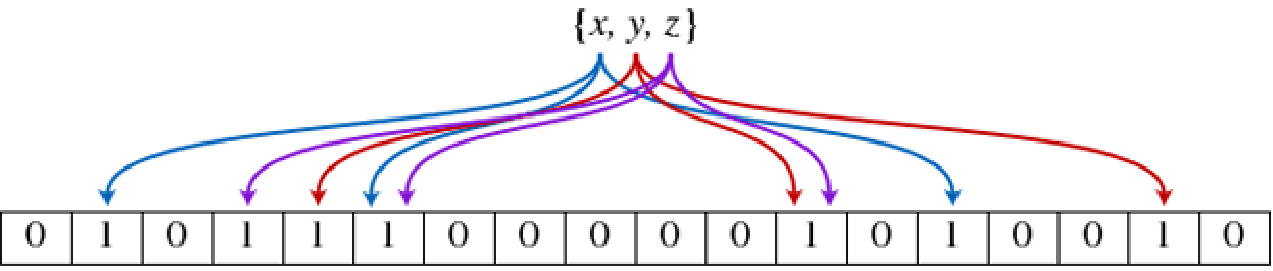
\includegraphics[width=7cm]{img/bloom-filter}}
\caption{Struttura filtri di bloom\label{bloom_filter}}
\end{figure}
Un filtro di Bloom consente di mappare un insieme di n elementi su un array di bit (posti inizialmente tutti a zero), applicando diverse funzioni hash ai vari elementi; viene così prodotto un array di bit che identificherà ogni singolo dato inserito, ponendo a 1 tutti i bit corrispondenti.  \linebreak
Per ritrovare il file sarà sufficiente  che il filtro calcoli nuovamente la funzione hash per l'elemento cercato e verificare che i bit relativi siano impostati a 1. Se l’esito del matching è negativo, allora l’elemento non appartiene sicuramente all’insieme. Se l’esito del lookup è positivo, è possibile che l’elemento appartenga all’insieme, con una certa probabilità di errore (si parla in questo caso di “falsi positivi”).\linebreak
Nonostante esista questa limitazione, la quantità di memoria occupata è minima rispetto al numero dei dati da condividere nella rete. Se un’operazione di lookup in un Bloom Filter porta ad un falso positivo, il risultato è semplicemente una query ad un nodo remoto per un oggetto che in realtà non possiede.\linebreak
Accettando una certa probabilità di errore (molto piccola se dimensionati opportunamente) si risparmia molto in occupazione di memoria. Nel progetto infatti il filtro viene creato a partire da un file contenente la lista dei nomi dei file condivisi e la dimensione del filtro è stata fissata a 100 byte. Mantenere intere liste di oggetti associate agli altri nodi della rete sarebbe proibitivo e anche il traffico in rete sarebbe stato maggiore, per questo motivo è stata scelta questa struttura per la rappresentazione dei file condivisi.\linebreak


\subsubsection{Protocolli di comunicazione}
Il peer comunica con due entità diverse: il server di bootstrap e il superpeer associato.\linebreak
Essendo la comunicazione con il server di bootstrap molto importante, in quanto permette al peer di accedere al sistema, il protocollo di comunicazione scelto è TCP. In questo modo il peer è sicuro di ricevere le informazioni necessarie per iniziare la sua corretta esecuzione.\linebreak
La comunicazione con il superpeer avviene invece in UDP, non perchè meno importante tale comunicazione, ma perchè il superpeer deve poter gestire un numero grande di peer e quindi è importante che la comunicazione sia leggera e che non ci siano troppe connessioni ad appesantire il lavoro svolto dal supernodo.\linebreak
I messaggi scambiati in udp sono strutturati in tre campi:
\begin{itemize}
\item Comand (4 byte)
\item Size (4 byte)
\item Data (dimensione variabile, indicata nel campo size)
\end{itemize}
L'unica eccezione a questa struttura sono i pacchetti UDP di whohas, i quali avranno un campo aggiuntivo per l'id della query.\linebreak
Non essendoci connessione tra peer e superpeer, non c'è garanzia sull'arrivo dei messaggi scambiati. Per offrire un minimo di sicurezza, ogni funzione che invia pacchetti UDP sul peer utilizza un timer per bloccare l'attesa della risposta da parte del superpeer. Il timer viene attivato chiamando una alarm e indicando il tempo dopo il quale sarà inviato il segnale di tipo SIGALRM; quando il peer riceve questo segnale attiverà una specifica funzione (alarm\_handler) che modificherà il valore della variabile var\_ack bloccando il ciclo in cui c'è la chiamata di ricezione.\linebreak
Se dopo lo scadere del timer non è stato ricevuto alcun messaggio, la funzione richiamerà se stessa per un numero finito di volte. In particolare è impostato ad un  massimo 5 volte il numero di tentativi possibili, e il valore di timeout dipenderà dal numero della chiamata ricorsiva in corso. Nel primo tentativo di invio il timeout è di 1 secondo e nelle chiamate successive aumenterà di un secondo ad ogni chiamata ricorsiva. In questo modo si fornisce un piccolo controllo di congestione, in quanto si evita la ritrasmissione ravvicinata di più pacchetti, dando più tempo al superpeer per rispondere in caso di congestione della rete.